\section{Malware Classification}
\label{sec:ssdeep}

Machine learning systems are just as good
as the data they consumed---One potential 
use case of the massive amount of data 
available on VirusTotal is to build 
machine learning models for applications
such as malware classifications and
clustering. In this section, we study
the question that {\em Is the data
provided by VirusTotal enough to support
classifications and clusterings tasks?}

Our study reveals both positive and
negative answers to this question---For
some classification tasks, we are able
to build an automatic classifier whose
accuracy is higher than 80\% by just
using the static signature provided by VirusTotal
and we expect the quality to keep increasing
given more data; on the other hand,
we identify some classification tasks
whose accuracy hardly beat random guesses.
We also identify a simple metrics
to predict whether a given task belongs
the high-quality category or the low-quality
category. We hope our study shed lights
on future design of signatures for malware
detection.

%Malware detectors mainly rely on signatures manually extracted by security researchers. 
%ssdeep only takes static binary executable as inputs. 
%If we can build malware detector based on ssdeep similarity, 
%We can reduce or even eliminate manual efforts in malware detection. 


\subsection{Data Collection}

\begin{table*}
  \centering
  \scriptsize
  {
  \begin{tabular}{clccc}
    \toprule
{\bf Index} & {\bf Microsoft Tag} & {\bf \# of Malwares} & {\bf \% of Tailing}  & {\bf \% of Distinct}\\
\midrule                                                                                                                                                                                                                                           
1  &  SoftwareBundler:Win32/Penzievs 	& 49380	     & 3.51\%  & 99.98\%\\
2  &  Adware:Win32/Hotbar               & 132161   & 1.88\%  & 99.98\%\\
3  &  TrojanDropper:Win32/Lamechi!rfn	& 39205	     & 0.01\%  & 6.13\%\\
4  &  Virus:Win32/Nabucur.D	            & 1190132  & 99.95\% & 100.00\%\\
5  &  Virus:Win32/Virut.BO	            & 84600	   & 21.84\% & 99.95\% \\
6  &  Worm:Win32/Mydoom.L@mm	        & 76259	     & 0\%     & 99.44\%\\
7  &  Virus:Win32/Ramnit.I              & 412052   & 3.07\%  & 96.76\%\\
8  &  Trojan:Win32/Dorv.A               & 54324    & 2.80\%  & 80.53\%\\
9  &  Trojan:Win32/Dynamer!ac           & 145402   & 65.17\% & 99.20\%\\
10 &  Virus:Win32/Ramnit.A              & 181524   & 26.79\% & 99.82\%\\   

\bottomrule
   \end{tabular}
   }
   \mycaption{tab:benchmark}{Benchmark Information.}
{\footnotesize{(Information for malwares used in our clustering and classification experiments. \# of Malwares: \# of distinct malwares we collected in each sampled malware group from 05/07/2016 to 09/06/2016. \% of Tailing: \% of tailing examples in each group. \% of Distinct: number of distinct ssdeep hash strings divided by group size.)}}
  %\nocaptionrule
  %\mycaption{tab:benchmark}{Malware Data Set.}
  %\footnotesize{(Information for malwares used in our clustering and classification experiments. \# of Malwares: \# of distinct malwares we collected in each sampled malware group from 05/07/2016 to 09/06/2016. \% of Tailing: \% of tailing examples for each group in the sampled 10000 malwares.)}
 %}
\end{table*}




Our study uses features based on ssdeep~\cite{ssdeep}, a program to compute fuzzy hashes. 
Similarity between calculated hash strings can serve as an estimation for similarity between the two original files. 
ssdeep hash strings are also provided for each submitted file with other metadata fields by \vt. 

We focus on classifying each malware into
different malware families. Because Microsoft 
has a good reputation in detecting PE malwares~\cite{SongAPsys2016}, we create training
data using its assignment. For each detected malware, 
Microsoft assigns it a tag, which contains type, platform, family, 
and variant information~\cite{microsoft}. 
We divide PE malwares detected by Microsoft engine into different groups, 
and malwares in the same group share the same Microsoft malware tag. 
We sample 10 groups, each of which with more than 10000 malwares.  
Microsoft tag and number of malwares in each sampled group we collected from \vt{} 
are shown in Table~\ref{tab:benchmark}. 
For each group, we sample 10000 malwares, and use these malwares in our following experiments. 

\subsection{Classification Accuracy}


We use knn~\cite{knn} as our classifier.
compare API of ssdeep takes two ssdeep hash strings as inputs, 
and return similarity between these two strings. 
We use 1 to minus ssdeep similarity to get ssdeep distance.  
We design several experiments to understand performance of 
the combination of knn and ssdeep 
distance (or similarity) when handling different classification tasks. 


We build a two-class classifier for each of the sampled groups. 
We use the 10000 sampled malwares from each group as positive examples. 
We sample 10000 benign files as negative examples. 
Benign files are files submitted to \vt{}, but are not labeled as malwares by any anti-virus engines. 
We randomly choose 5000 malwares and 5000 benign files for training, 
and use the left malwares and benign files for testing. 
We run cross validation for k from 1 to 10 to pick up best k, 
and use the best k to test knn with the testing set. 

The best k used for testing and classification results are shown in Table~\ref{tab:results}.
We see that 1 is always the best k value for testing, except for two groups.
For five out of
ten malware families, we achieve an accuracy higher than 80\%.
On the other hand, for
families such as ``Virus:Win32/Nabucur.D'',
the classification accuracy are significant
lower. We get an accuracy of 59\% when
the accuracy of random guesses would be 50\%.
For this classifier, we think there are quite limited malwares and benign files similar to instances in testing set. 

We also build a ten-class classifier.
We randomly choose 2000 malwares from each group, 
and put half of them in training set, and half of them in testing set. 
We also run cross validation to pick up best k from 1 to 10. 
The accuracy on the testing set with best k value 1 is 70.15\%. 

\begin{figure*}
\centering
\subfloat[Group 1]{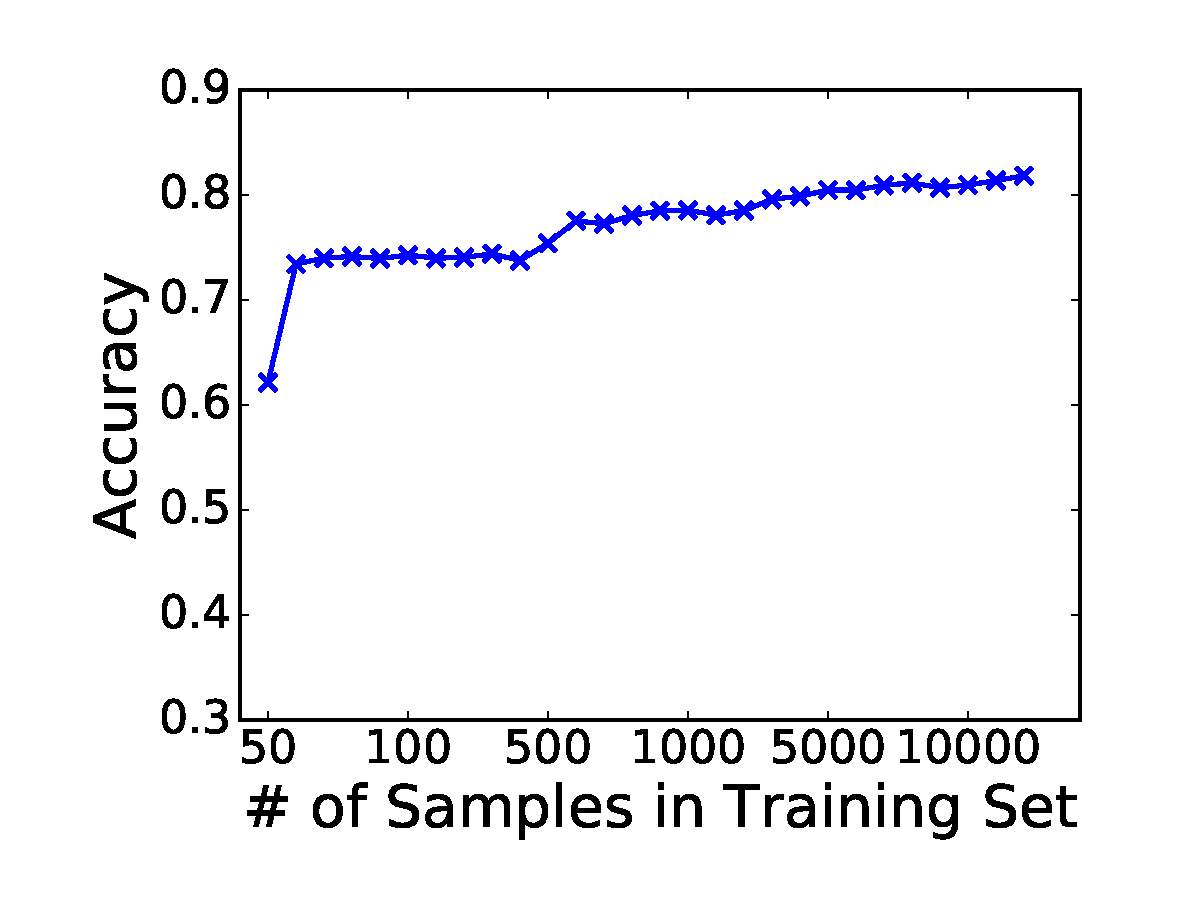
\includegraphics[width=0.16\linewidth]{figure/svm/0}\label{fig:moredata1}} 
\subfloat[Group 2]{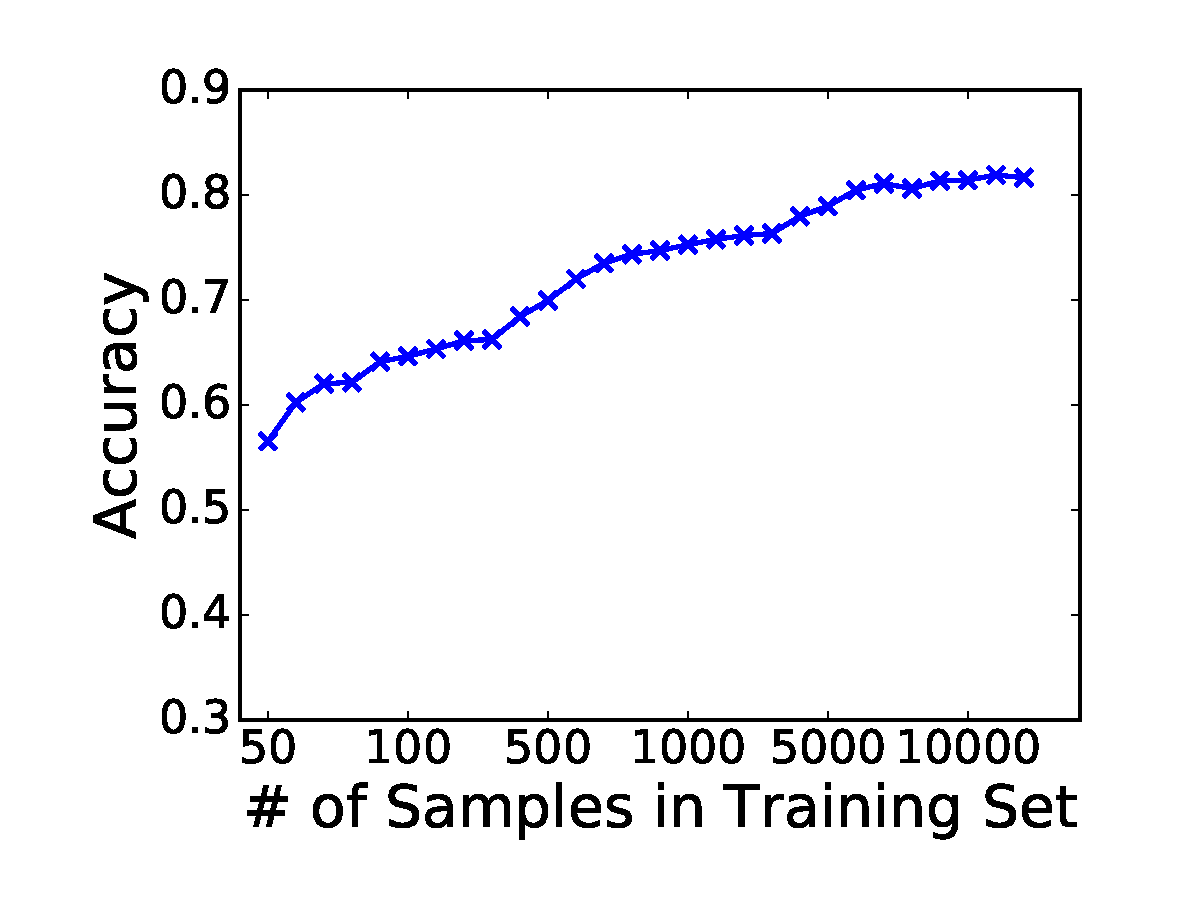
\includegraphics[width=0.16\linewidth]{figure/svm/1}\label{fig:moredata2}}
\subfloat[Group 3]{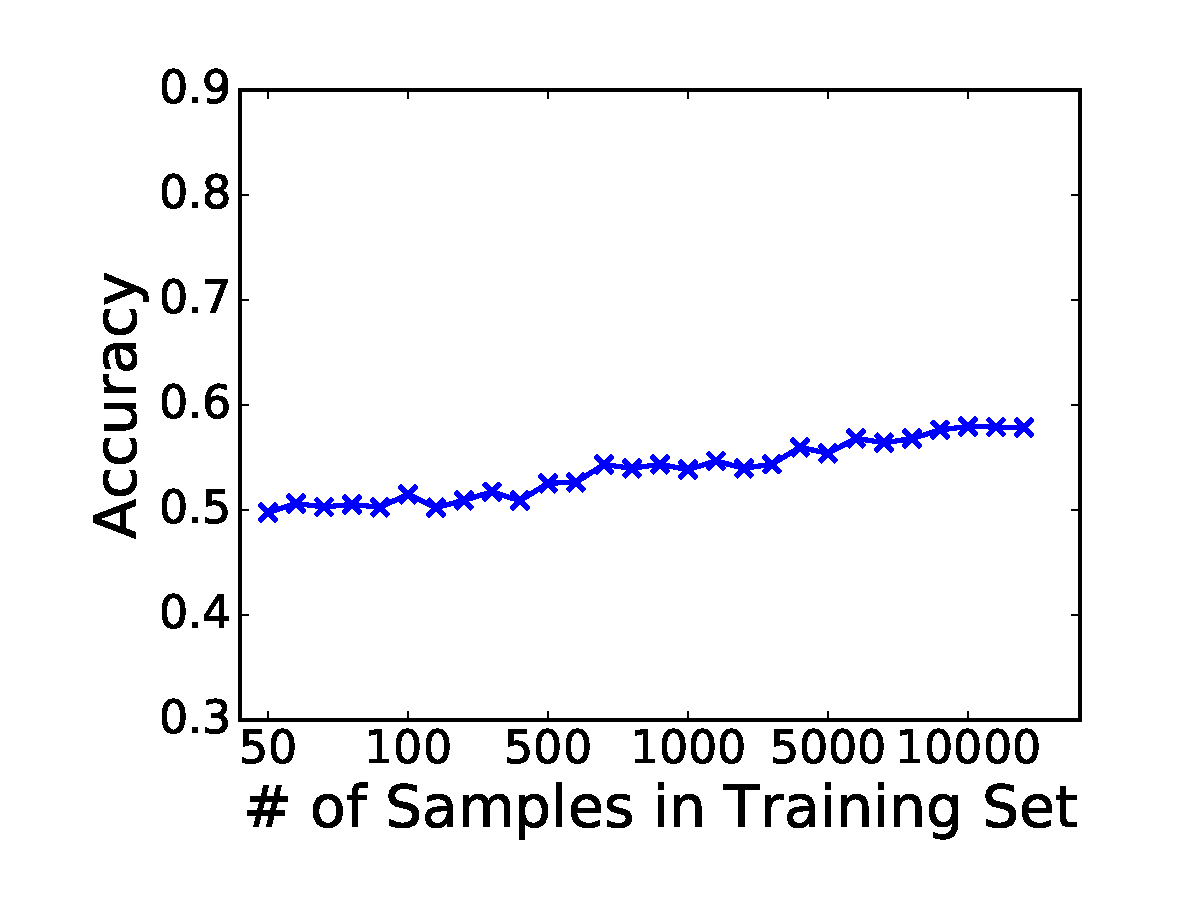
\includegraphics[width=0.16\linewidth]{figure/svm/2}\label{fig:moredata3}} 
\subfloat[Group 4]{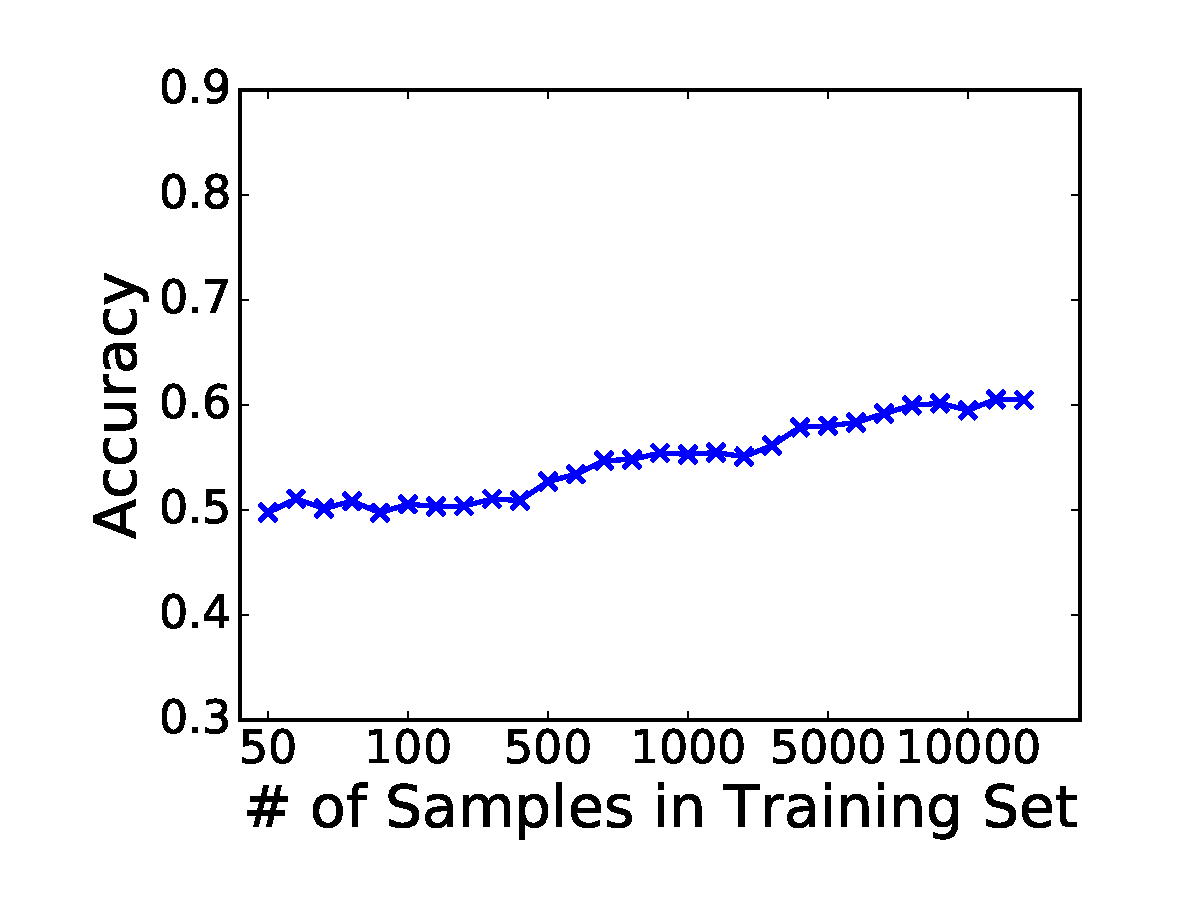
\includegraphics[width=0.16\linewidth]{figure/svm/3}\label{fig:moredata4}}
\subfloat[Group 5]{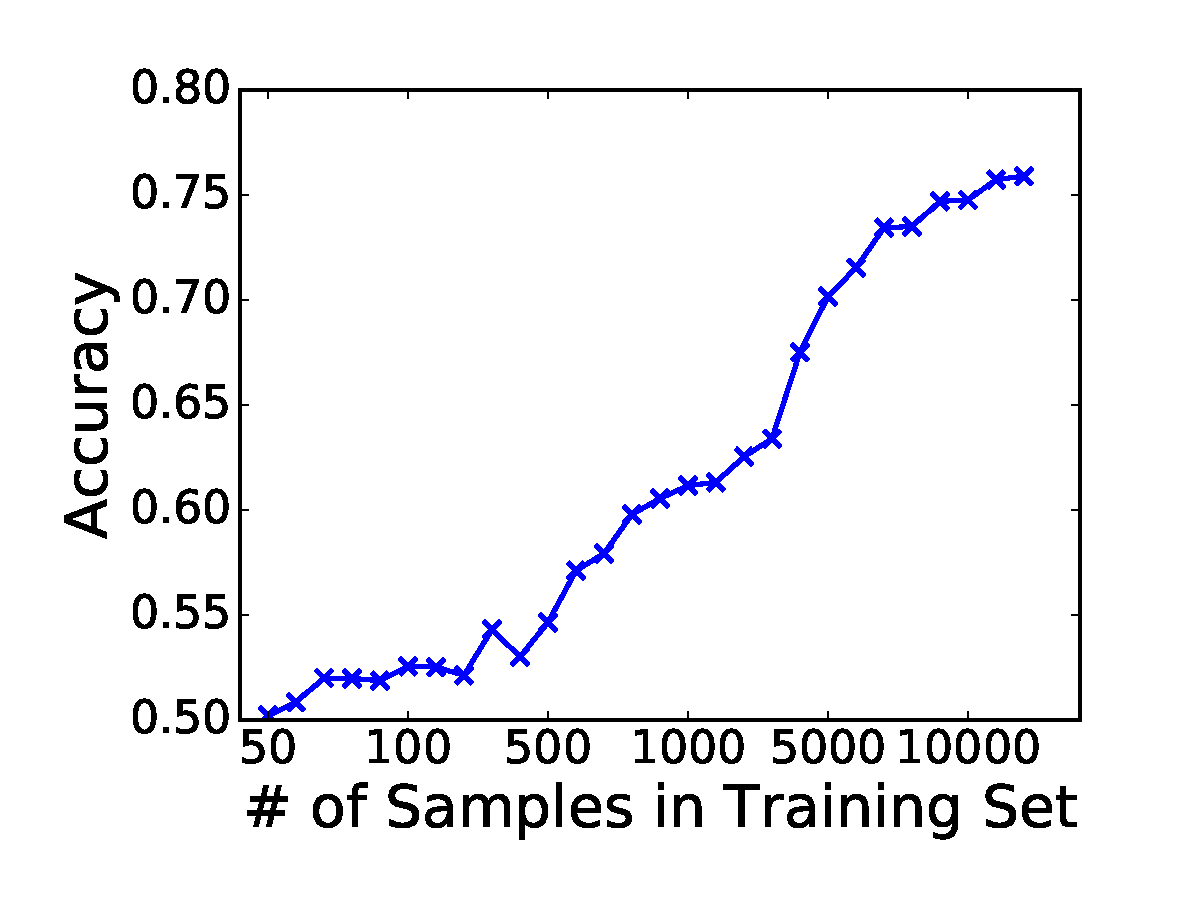
\includegraphics[width=0.16\linewidth]{figure/svm/4}\label{fig:moredata5}} \\ 

\subfloat[Group 6]{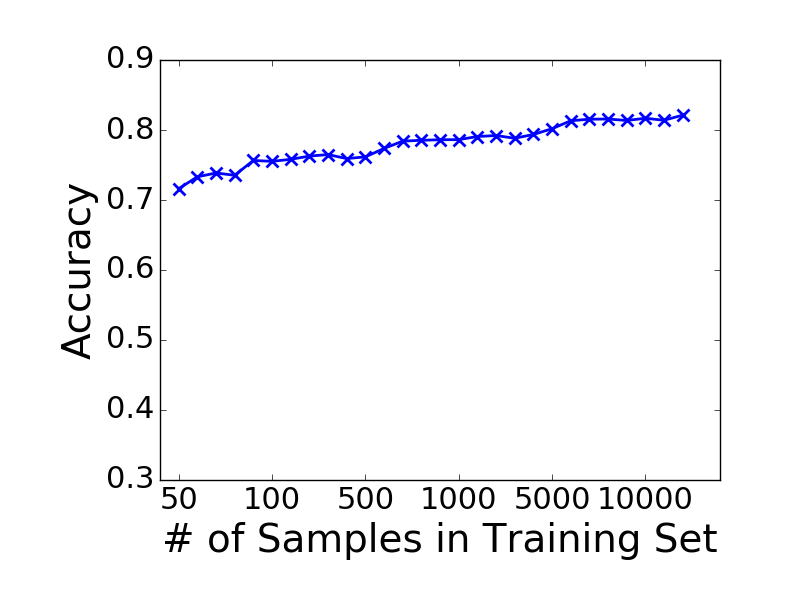
\includegraphics[width=0.16\linewidth]{figure/svm/5}\label{fig:moredata6}} 
\subfloat[Group 7]{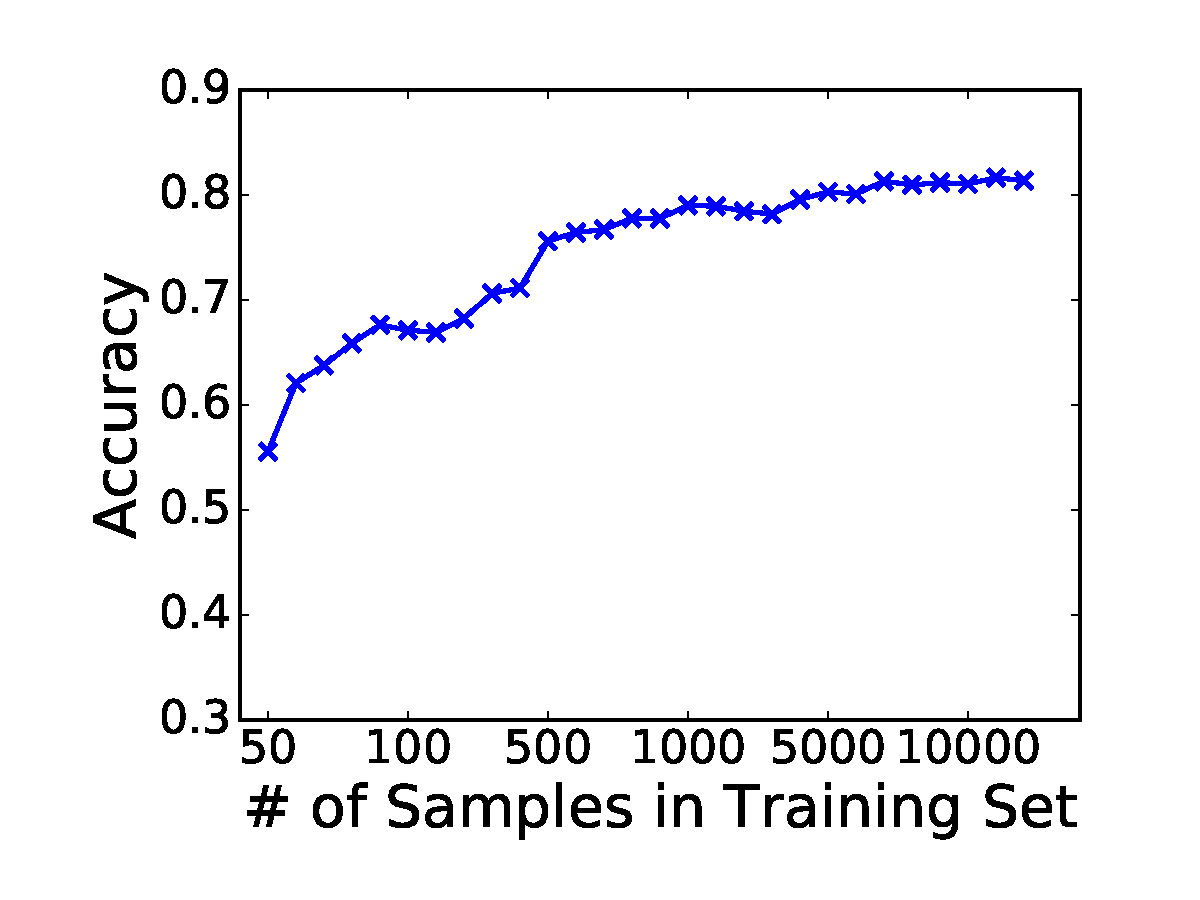
\includegraphics[width=0.16\linewidth]{figure/svm/6}\label{fig:moredata7}}
\subfloat[Group 8]{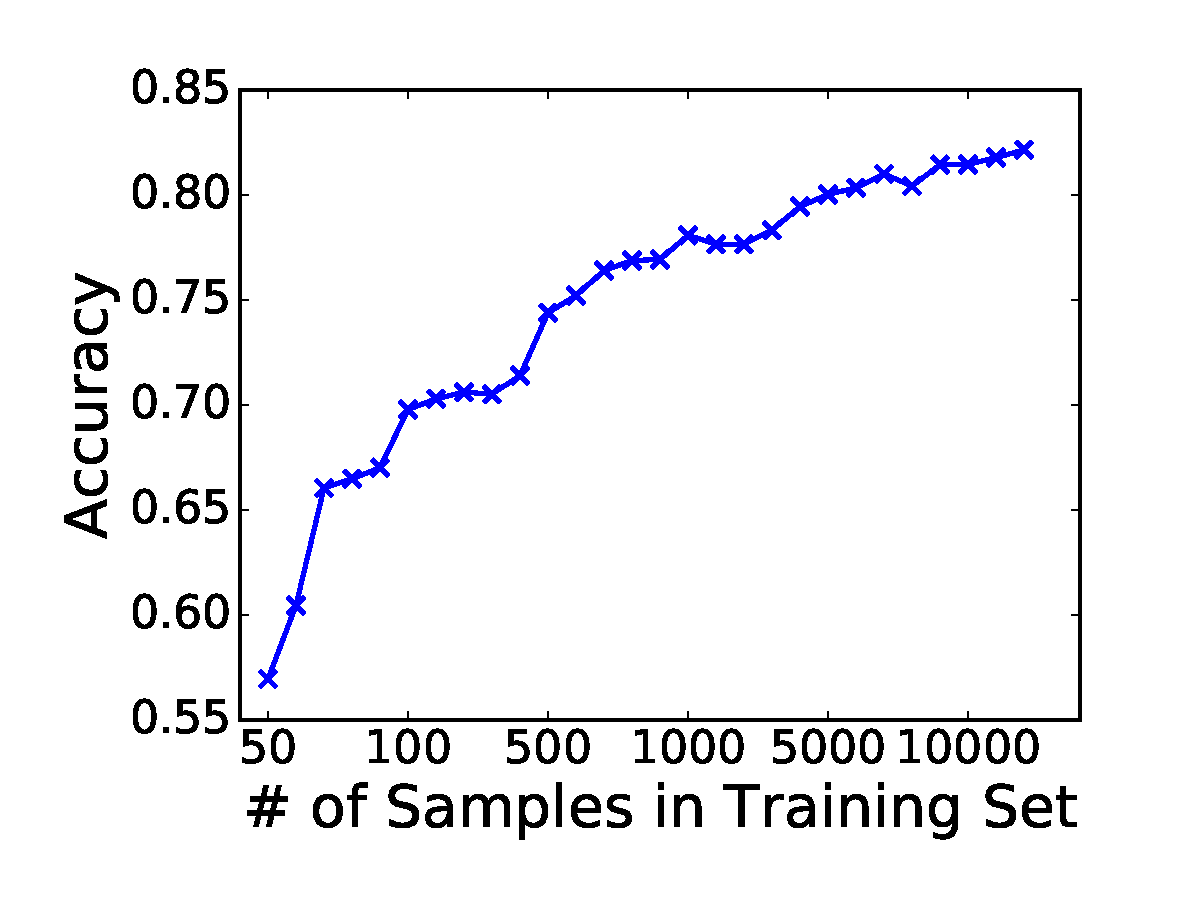
\includegraphics[width=0.16\linewidth]{figure/svm/7}\label{fig:moredata8}} 
\subfloat[Group 9]{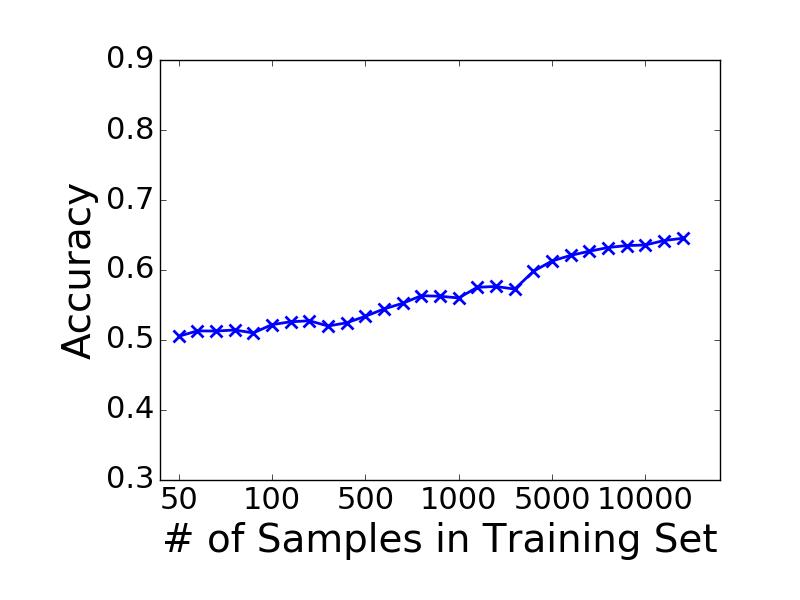
\includegraphics[width=0.16\linewidth]{figure/svm/8}\label{fig:moredata9}}
\subfloat[Group 10]{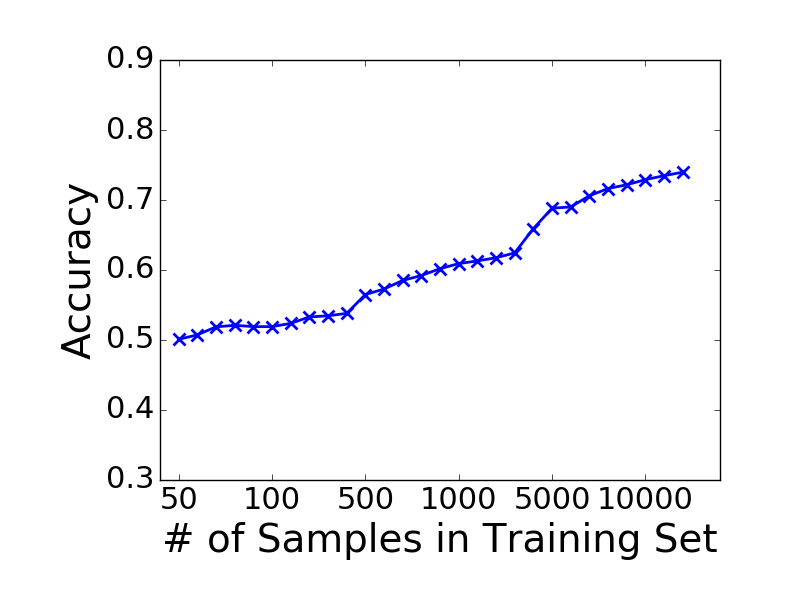
\includegraphics[width=0.16\linewidth]{figure/svm/9}\label{fig:moredata10}}
\subfloat[10-class]{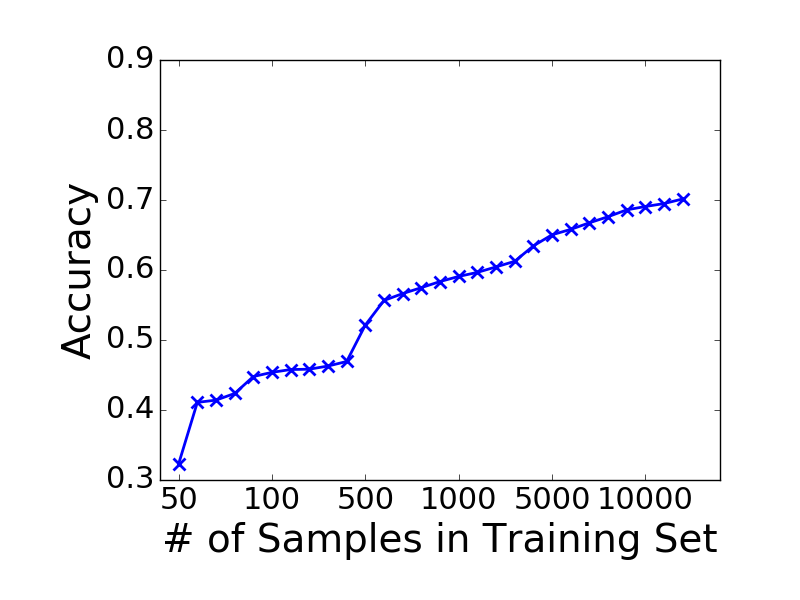
\includegraphics[width=0.16\linewidth]{figure/svm/10}\label{fig:moredata11}}
\caption{How accuracy changes with more data in traning set. 
{\footnotesize{(Figure~\ref{fig:moredata1} - Figure~\ref{fig:moredata10} show how accuracy of each two-class classifier changes 
with the size of training set changing from 50 to 10000. 
Figure~\ref{fig:moredata11} shows how accuracy of the ten-class classifier changes with the size of training set increaing from 50 to 10000. )}}} 
\label{fig:moredata} 
\end{figure*} 



\begin{figure}[t!]
\begin{center}
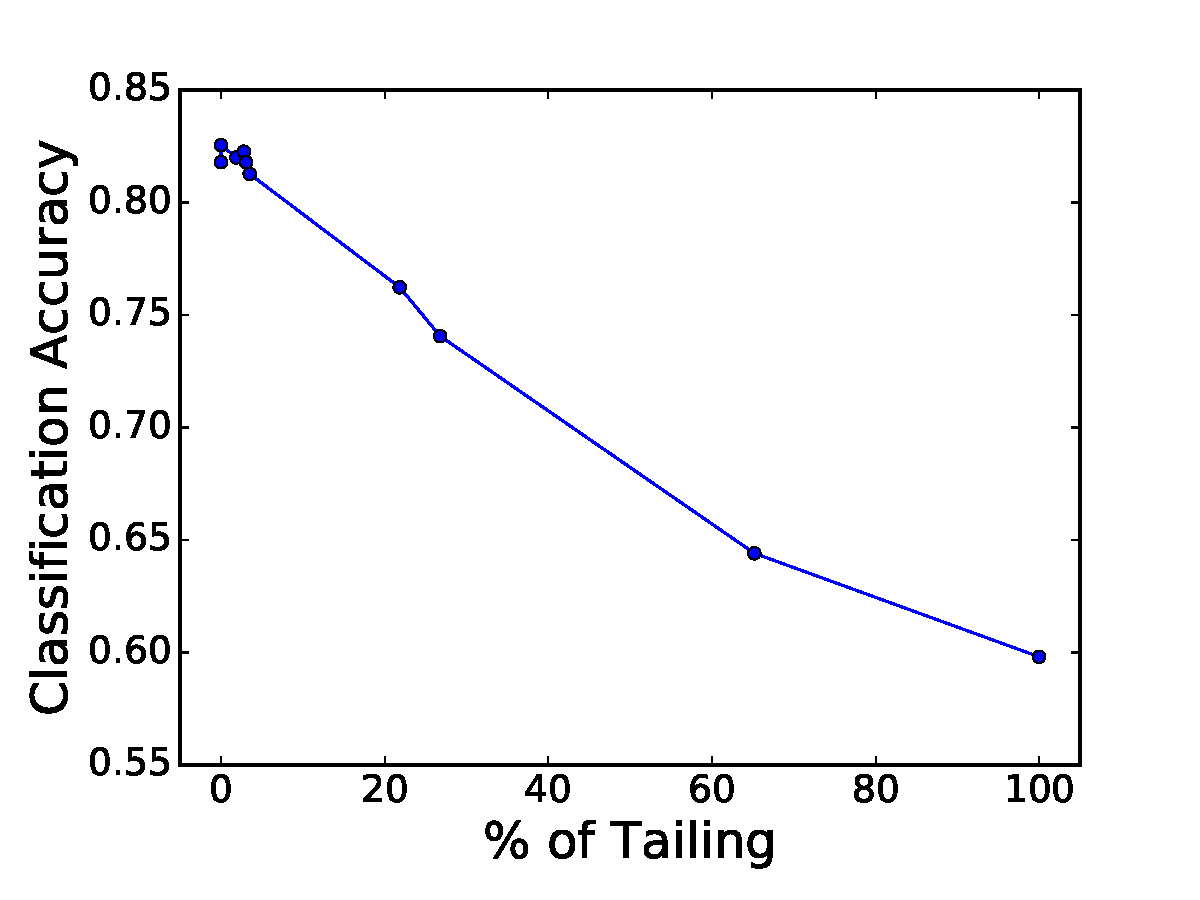
\includegraphics[width=2.5in]{figure/accuracy}
\mycaption{fig:accuracy}{The relation between classifer's accuracy and the percentage of tailing.}
{\footnotesize{(How classifier's accuracy changes with the percentage of tailing.)}}
\end{center}
%\vspace{-0.25in}
\end{figure}




For each designed classifier, we investigate 
how the size of training set influences its accuracy.
We keep test sets unchanged.  
We increase the size of training set from 50 to 10000, 
while keeping the number of examples from different classes equal to each other.  
We use the best k value got from cross validation in earlier experiments.
How accuracy changes with the size of training set is shown in Figure~\ref{fig:moredata}. 
Accuracy increases as we have more data for all these classifier. 

We also design several other two-class classification tasks. 
We classify malwares from Group 7 with malwares from Group 10. 
They are malwares from the same class Ramnit, but in different variant. 
The precision is 85.31\%. 
We classify malwares from Group 3 with malwares from Group 7 and Group 10, 
and classify malwares from Group 5 with malwares from Group 7 and Group 10. 
These two classifications try to classify malwares in different families. 
We get precision 94.15\% and 85.82\%, respectively. 
We classify malwares from Group 8 and Group 9 with malwares from Group 4, Group 5, Group 7 and Group 10, 
because we want to classify malwares in different types, one is Trojan and the other is Virus. We get precision 77.04\%. 
All experimental setting are the same as what we did during classifying malwares in each group with benign files. 

\paragraph*{Discussion: Tailing Malwares}

We identify one metrics to predict whether
a classification task falls into the
high-accuracy category or low-accuracy
category. The intuition is that the probability
that a given sample has similar samples in
the training set is a proxy of the upper bound
of accuracy that we can expect. Therefore,
we compute the percentage of tailing malwares in each group--We call malwares, which have 0 similarity with all the other samples in the same group, as tailing malwares. 
The percentage of tailing malwares for each sampled group is also shown in Table~\ref{tab:benchmark}. 
How accuracy changes with the percentage of tailing for each two-class classifier is shown in Figure~\ref{fig:accuracy}. 

%\ce{LINHAI, ADD IN THAT \#TRAILING-VS.ACCURACY FIGURE AND ARGUE ABOUT CORRELATION HERE.}

\paragraph*{Discussion: Challenge of Applying Nystrom Methods for Kernel Machines}

%\begin{table*}
\centering
\footnotesize
{
\begin{tabular}{cccccccccccc}
 \toprule
  & \multicolumn{9}{c}{Clustering} &\multicolumn{2}{c}{Classification}\\
\cline{1-1}
\cline{2-10}
\cline{11-12}
 \bf{Index}             & {\bf 0.1}  & {\bf 0.2} & {\bf 0.3} & {\bf 0.4} & {\bf 0.5}  & {\bf 0.6} & {\bf 0.7} & {\bf 0.8} & {\bf 0.9} & {\bf Best k} & {\bf Precision} \\
              \midrule  
          1   & 2483       & 575       &  503      &   456     & 443        & 381       & 356       & 356       & 356       &     1        & 81.27\%  \\
          2   & 4192       & 762       &  635      &   588     & 580        & 534       & 526       & 526       & 526       &     1        & 82\%     \\
          3   &  5         & 4         &  3        &    2      & 2          & 2         & 2         & 2         & 2         &     1        & 82.55\%  \\
          4   & 10000      & 9999      & 9998      & 9997      & 9997       & 9997      & 9997      & 9997      & 9997      &     2        & 59.81\%  \\
          5   & 8688       & 7727      & 6630      & 5462      & 4699       & 3690      & 3103      & 3028      & 3028      &     1        & 76.23\%   \\
          6   & 5807       & 3915      & 1590      & 373       & 18         & 1         & 1         & 1         & 1         &     3        & 81.79\%   \\
          7   & 5429       & 3651      & 2703      & 1615      & 726        & 400       & 369       & 362       & 362       &     1        & 81.79\%   \\
          8   & 2721       & 1400      & 871       & 642       & 549        & 420       & 399       & 396       & 396       &     1        & 82.26\%    \\
          9   & 8500       & 8199      & 8012      & 7808      & 7597       & 7327      & 7171      & 7150      & 7150      &     1        & 64.41\%    \\
          10  & 8075       & 7241      & 6343      & 5193      & 4382       & 3800      & 3506      & 3480      & 3480      &     1        & 74.06\%    \\

\bottomrule
\end{tabular}
}
 \mycaption{tab:results}{Clustering and Classification Results.}
{\footnotesize{(Numbers of resulting clusters under distance threshold from 0.1 to 0.9 are shown in \bf{Clustering} column. K with best precision during cross validation and precision of knn with best k are shown in \bf{Classification} column.)}}
%\caption{Clustering and Classification Results. \footnotesize{(Numbers of resulting clusters under distance threshold from 0.1 to 0.9 are shown in \bf{Clustering} column.
%K with best precision during cross validation and precision of knn with best k are shown in \bf{Classification} column.)}
%}
\end{table*}

Our previous experiment uses knn classifier.
In this section, we discuss the potential of using
more sophisticated classifiers such as
support vector machines. One challenge
of applying kernel machines is to
approximate the kernel matrix whose
size is quadratic to the number of samples
in the training set. Nystrom Methods~\cite{clustering-purpose} are popular ways to
approximate a kernel matrix with clusters.

To understand the potential of applying Nystrom Methods, we run hierarchical clustering~\cite{hcluster} on our data.
Hierarchical clustering starts with each instance as a cluster, 
and then it iteratively merge two clusters with minimum distance 
until distance threshold or cluster number threshold is reached. 
We use distance as threshold. 
Given two malwares, 
we use 1 to minus their ssdeep similarity to calculate distance between the two malwares. 
We calculate single linkage distance as distance between two clusters. 
Single linkage
distance~\cite{single-link} when we need to compute distance between two clusters. 

We change distance threshold from 0.1 to 0.9, 
and count resulting clusters under each experiment. 
Experimental results are shown in Table~\ref{tab:results}. 
As we increase distance threshold, the number of resulting clusters decreases for each sampled group. 
The number of resulting clusters is always bounded by the number of tailing in each group. 
If we want to change a ssdeep hash string to a feature vector, 
based on distance of the string to the center of all clusters in training set, 
the size of the resulting feature vector would have a very large variance across different malware groups. 
\ce{This illustrates a challenge of directly applying
classic Nystrom method, however, we believe
it is possible to develop new approaches to
accommodate this observation in the future.}


%\subsection{Classification Experiments}


\subsection{Discussion}

\ce{ LINHAI 
1. Future work about indexing ssdeep string
2. Upper bound
3. More data better results
4. Need human effort or dynamic information 
5. security of using ssdeep
}





